\documentclass[12pt]{article} % use larger type; default would be 10pt

\usepackage{pgfplots}
\usetikzlibrary{calc}
\usetikzlibrary{arrows}
\usetikzlibrary{patterns}
\usetikzlibrary{calc,intersections,through,backgrounds}
\usetikzlibrary{decorations.pathreplacing}
        \usepackage{xcolor} 
        \newcommand\degree[0]{^{\circ}}
        \newcommand\abs[1]{\left|#1\right|}
\usepackage{amsmath}
        \newcommand{\alert}[1]{\boldsymbol{\color{magenta}{#1}}}
        \newcommand{\blert}[1]{\boldsymbol{\color{blue}{#1}}}

\title{Play with TikZ}
\author{Just Us}
%\date{} % Activate to display a given date or no date (if empty),
         % otherwise the current date is printed 

\begin{document}
\maketitle

\section{Chap 6 Section 1}




fig-6-1-ex2


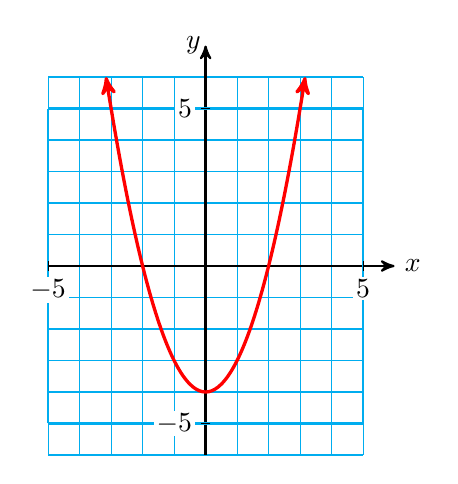
\begin{tikzpicture}[scale=.4]
\def\delx{0};
\draw[cyan] (-5,-6) grid (5,6);
\draw[black, thick, ->, >=stealth'] (-5,0)--(6,0) node[right]{$x$};
\draw[black, thick, ->, >=stealth'] (0,-6)--++(0,13) node[left, xshift=2]{$y$};
\foreach \x  in  {-5, 5} {
 \draw[cyan, thick] ({\x},-5) --++(0,10);
 \draw[cyan, thick] ({-5},\x) --++(10,0);
 \draw[black] ({\x},.15) --++(0,-.3) node[below, yshift=-2, fill=white, inner sep=1]   {$\x$};
 \draw[black] ({.15},\x) --++(-.3,0) node[left, xshift=-2, fill=white, inner sep=1]   {$\x$};
}
\draw[samples=65,domain={-sqrt(10)}:{sqrt(10)},smooth,variable=\x,red, very thick,<->, >=stealth'] plot ({\x},{(\x)^2-4});
\end{tikzpicture}
\newline



fig-6-1-2


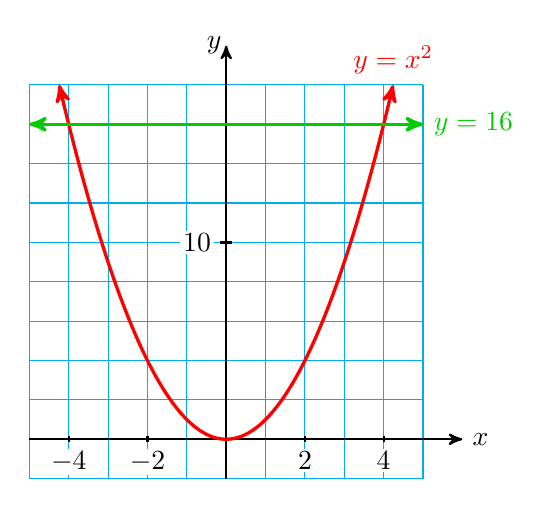
\begin{tikzpicture}[xscale=.5, yscale=.25]
\def\delx{0};
\draw[cyan] (-5,-2) grid[ystep=2] (5,18);
\draw[black, thick, ->, >=stealth'] (-5,0)--(6,0) node[right]{$x$};
\draw[black, thick, ->, >=stealth'] (0,-2)--++(0,22) node[left, xshift=2]{$y$};
\foreach \x  in  {-4, -2, 2, 4} {
 \draw[black, thick] ({\x},.15) --++(0,-.3) node[below, yshift=-2, fill=white, inner sep=1]   {$\x$};
}
\draw[black, thick] (.15,10) --++(-.3,0) node[left, xshift=-2, fill=white, inner sep=1]   {$10$};
\draw[samples=65,domain={-sqrt(18)}:{sqrt(18)},smooth,variable=\x,red, very thick,<->, >=stealth'] plot ({\x},{(\x)^2}) node[above] {$y=x^2$};;
\draw[green!80!black, very thick, <->, >=stealth'] (-5,16)--(5,16) node[right] {$y=16$};
\end{tikzpicture}
\newline


fig-6-1-3


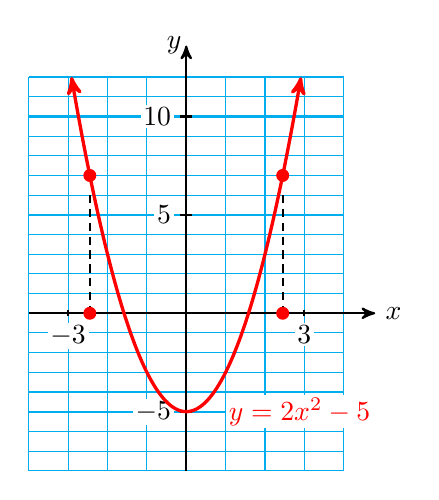
\begin{tikzpicture}[xscale=.5, yscale=.25]
\draw[cyan] (-4,-8) grid (4,12);
\draw[black, thick, ->, >=stealth'] (-4,0)--(4.8,0) node[right]{$x$};
\draw[black, thick, ->, >=stealth'] (0,-8)--(0,13.6) node[left, xshift=2]{$y$};
\foreach \x  in  {-3,3} {
 \draw[black, thick] ({\x},.15) --++(0,-.3) node[below, yshift=-2, fill=white, inner sep=1]   {$\x$};
}
\foreach \x  in  {-5,5,10} {
 \draw[cyan,thick] (-4,\x)--++(8,0);
 \draw[black, thick] (.15,\x) --++(-.3,0) node[left, xshift=-2, fill=white, inner sep=1]   {$\x$};
}
\draw[samples=65,domain={-sqrt(8.5)}:{sqrt(8.5)},smooth,variable=\x,red, very thick,<->, >=stealth'] plot ({\x},{2*(\x)^2-5});
\node[right, text=red, fill=white, inner sep=1] at (1,-5) {$y=2x^2-5$};
\draw[black,thick, densely dashed] ({-sqrt(6)}, 6) --++(0,-6);
\draw[black,thick, densely dashed] ({sqrt(6)}, 6) --++(0,-6);
\filldraw[red] ({sqrt(6)},7) ellipse (1.5mm and 3mm);
\filldraw[red] ({-sqrt(6)},7) ellipse (1.5mm and 3mm);
\filldraw[red] ({sqrt(6)},0) ellipse (1.5mm and 3mm);
\filldraw[red] ({-sqrt(6)},0) ellipse (1.5mm and 3mm);
\end{tikzpicture}
\newline


fig-6-1-ex5


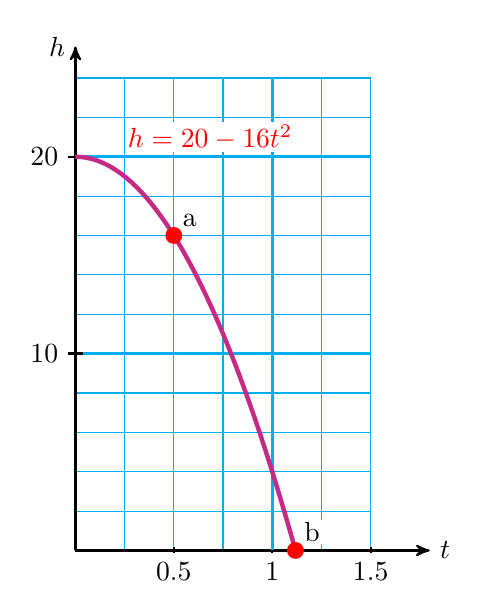
\begin{tikzpicture}[xscale=2.5, yscale=.25]
\draw[cyan] (0,0) grid[xstep=1/4, ystep=2] (3/2,24);
\draw[black, thick, ->, >=stealth'] (0,0)--(1.8,0) node[right]{$t$};
\draw[black, thick, ->, >=stealth'] (0,0)--(0,25.6) node[left]{$h$};
\foreach \x  in  {0.5,1,1.5} {
 \draw[black, thick] ({\x},.15) --++(0,-.3) node[below, yshift=-2, fill=white, inner sep=1]   {$\x$};
}
\draw[cyan, very thick] (1,0)--++(0,24);
\foreach \x  in  {10,20} {
 \draw[cyan, very thick] (0,\x)--++(1.5,0);
\draw[black, thick] (.04,\x) --++(-.08,0) node[left, xshift=-2, fill=white, inner sep=1]   {$\x$};
}
\draw[samples=65,domain=0:{sqrt(1.25)},smooth,variable=\x,magenta!80!black, ultra thick] plot ({\x},{20-16*(\x)^2});
\node[right, text=red, fill=white, inner sep=1] at (0.25,21) {$h=20-16t^2$};
\filldraw[red] (0.5,16) ellipse (.4mm and 4mm) node[above right, xshift=2, yshift=2, fill=white, inner sep=1, text=black] {a};
\filldraw[red] ({sqrt(1.25)},0) ellipse (.4mm and 4mm) node[above right, xshift=2, yshift=2, fill=white, inner sep=1, text=black] {b};
\end{tikzpicture}
\newline


hp-6-1-2


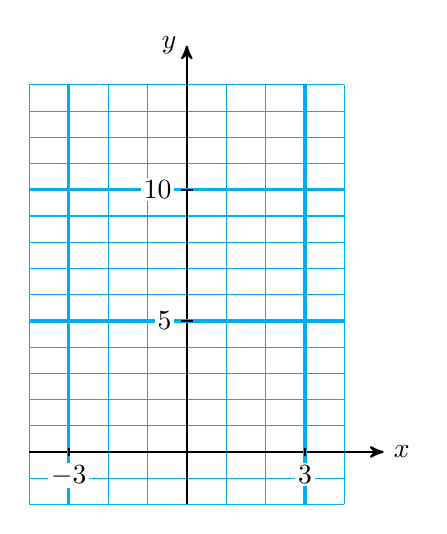
\begin{tikzpicture}[xscale=.5, yscale=.333]
\draw[cyan] (-4,-2) grid (4,14);
\draw[black, thick, ->, >=stealth'] (-4,0)--(5,0) node[right]{$x$};
\draw[black, thick, ->, >=stealth'] (0,-2)--(0,15.5) node[left]{$y$};
\foreach \x  in  {-3,3} {
\draw[cyan, very thick] (\x,-2)--++(0,16);
 \draw[black, thick] ({\x},.15) --++(0,-.3) node[below, yshift=-2, fill=white, inner sep=1]   {$\x$};
}
\foreach \x  in  {5,10} {
 \draw[cyan, very thick] (-4,\x)--++(8,0);
\draw[black, thick] (.15,\x) --++(-.3,0) node[left, xshift=-2, fill=white, inner sep=1]   {$\x$};
}
\end{tikzpicture}
\newline


hp-6-1-3


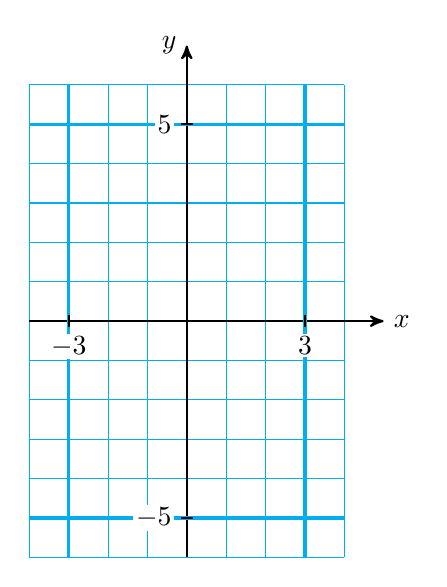
\begin{tikzpicture}[scale=.5]
\draw[cyan] (-4,-6) grid (4,6);
\draw[black, thick, ->, >=stealth'] (-4,0)--(5,0) node[right]{$x$};
\draw[black, thick, ->, >=stealth'] (0,-6)--(0,7) node[left]{$y$};
\foreach \x  in  {-3,3} {
\draw[cyan, very thick] (\x,-6)--++(0,12);
 \draw[black, thick] ({\x},.15) --++(0,-.3) node[below, yshift=-2, fill=white, inner sep=1]   {$\x$};
}
\foreach \x  in  {-5,5} {
 \draw[cyan, very thick] (-4,\x)--++(8,0);
\draw[black, thick] (.15,\x) --++(-.3,0) node[left, xshift=-2, fill=white, inner sep=1]   {$\x$};
}
\end{tikzpicture}
\newline


hp-6-1-3ans


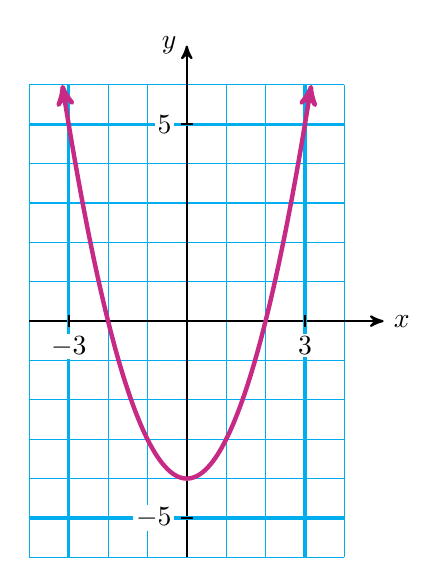
\begin{tikzpicture}[scale=.5]
\draw[cyan] (-4,-6) grid (4,6);
\draw[black, thick, ->, >=stealth'] (-4,0)--(5,0) node[right]{$x$};
\draw[black, thick, ->, >=stealth'] (0,-6)--(0,7) node[left]{$y$};
\foreach \x  in  {-3,3} {
\draw[cyan, very thick] (\x,-6)--++(0,12);
 \draw[black, thick] ({\x},.15) --++(0,-.3) node[below, yshift=-2, fill=white, inner sep=1]   {$\x$};
}
\foreach \x  in  {-5,5} {
 \draw[cyan, very thick] (-4,\x)--++(8,0);
\draw[black, thick] (.15,\x) --++(-.3,0) node[left, xshift=-2, fill=white, inner sep=1]   {$\x$};
}
\draw[samples=65,domain={-sqrt(10)}:{sqrt(10)},smooth,variable=\x,magenta!80!black, ultra thick, <->, >=stealth'] plot ({\x},{(\x)^2-4});
\end{tikzpicture}
\newline


hp-6-1-5ans


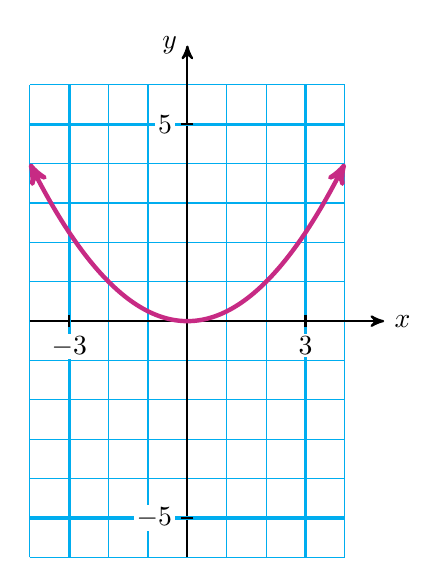
\begin{tikzpicture}[scale=.5]
\draw[cyan] (-4,-6) grid (4,6);
\draw[black, thick, ->, >=stealth'] (-4,0)--(5,0) node[right]{$x$};
\draw[black, thick, ->, >=stealth'] (0,-6)--(0,7) node[left]{$y$};
\foreach \x  in  {-3,3} {
\draw[cyan, very thick] (\x,-6)--++(0,12);
 \draw[black, thick] ({\x},.15) --++(0,-.3) node[below, yshift=-2, fill=white, inner sep=1]   {$\x$};
}
\foreach \x  in  {-5,5} {
 \draw[cyan, very thick] (-4,\x)--++(8,0);
\draw[black, thick] (.15,\x) --++(-.3,0) node[left, xshift=-2, fill=white, inner sep=1]   {$\x$};
}
\draw[samples=65,domain=-4:4,smooth,variable=\x,magenta!80!black, ultra thick, <->, >=stealth'] plot ({\x},{0.25*(\x)^2});
\end{tikzpicture}
\newline


hp-6-1-7aans


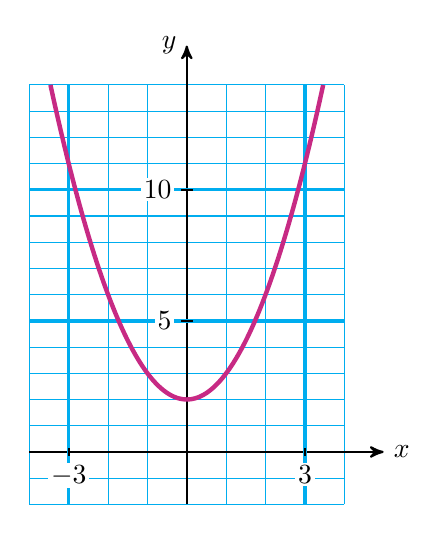
\begin{tikzpicture}[xscale=.5, yscale=.333]
\draw[cyan] (-4,-2) grid (4,14);
\draw[black, thick, ->, >=stealth'] (-4,0)--(5,0) node[right]{$x$};
\draw[black, thick, ->, >=stealth'] (0,-2)--(0,15.5) node[left]{$y$};
\foreach \x  in  {-3,3} {
\draw[cyan, very thick] (\x,-2)--++(0,16);
 \draw[black, thick] ({\x},.15) --++(0,-.3) node[below, yshift=-2, fill=white, inner sep=1]   {$\x$};
}
\foreach \x  in  {5,10} {
 \draw[cyan, very thick] (-4,\x)--++(8,0);
\draw[black, thick] (.15,\x) --++(-.3,0) node[left, xshift=-2, fill=white, inner sep=1]   {$\x$};
}
\draw[samples=65,domain={-sqrt(12)}:{sqrt(12)},smooth,variable=\x,magenta!80!black, ultra thick] plot ({\x},{2+(\x)^2});
\end{tikzpicture}
\newline


hp-6-1-25


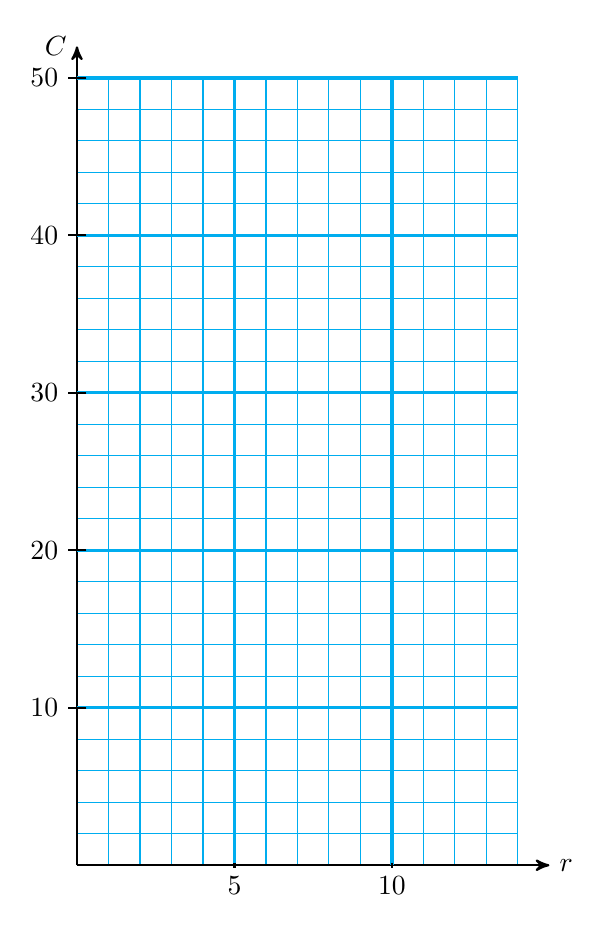
\begin{tikzpicture}[xscale=.4, yscale=.2]
\draw[cyan] (0,0) grid[ystep=2] (14,50);
\draw[black, thick, ->, >=stealth'] (0,0)--(15,0) node[right]{$r$};
\draw[black, thick, ->, >=stealth'] (0,0)--(0,52) node[left]{$C$};
\foreach \x  in  {5,10} {
\draw[cyan, very thick] (\x,0)--++(0,50);
 \draw[black, thick] ({\x},.15) --++(0,-.3) node[below, yshift=-2, fill=white, inner sep=1]   {$\x$};
}
\foreach \x  in  {10,20,...,50} {
 \draw[cyan, very thick] (0,\x)--++(14,0);
\draw[black, thick] (.3,\x) --++(-.6,0) node[left, xshift=-2, fill=white, inner sep=1]   {$\x$};
}
\end{tikzpicture}
\newline


hp-6-1-25aans


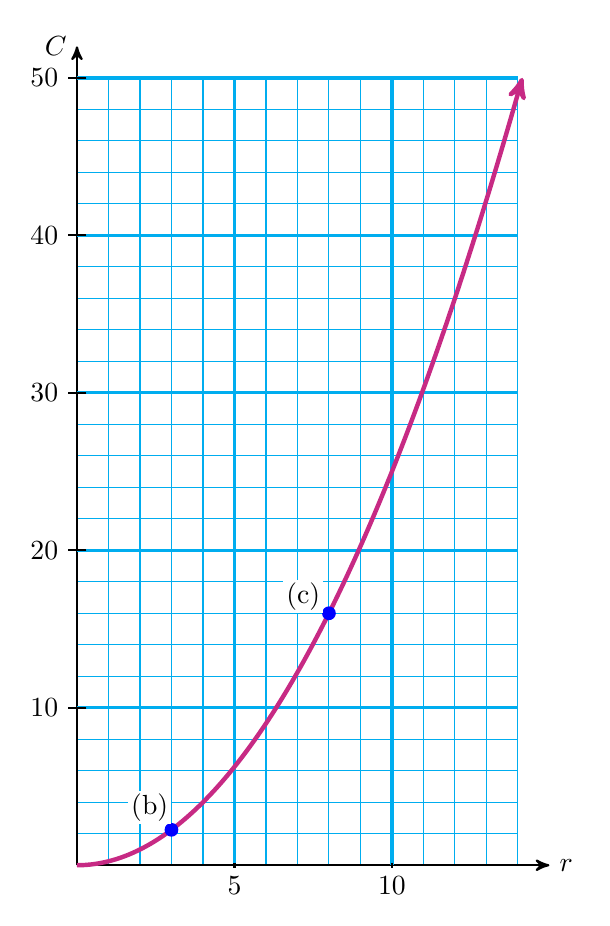
\begin{tikzpicture}[xscale=.4, yscale=.2]
\draw[cyan] (0,0) grid[ystep=2] (14,50);
\draw[black, thick, ->, >=stealth'] (0,0)--(15,0) node[right]{$r$};
\draw[black, thick, ->, >=stealth'] (0,0)--(0,52) node[left]{$C$};
\foreach \x  in  {5,10} {
\draw[cyan, very thick] (\x,0)--++(0,50);
 \draw[black, thick] ({\x},.15) --++(0,-.3) node[below, yshift=-2, fill=white, inner sep=1]   {$\x$};
}
\foreach \x  in  {10,20,...,50} {
 \draw[cyan, very thick] (0,\x)--++(14,0);
\draw[black, thick] (.3,\x) --++(-.6,0) node[left, xshift=-2, fill=white, inner sep=1]   {$\x$};
}
\draw[samples=65,domain=0:{sqrt(200)},smooth,variable=\x,magenta!80!black, ultra thick, ->, >=stealth'] plot ({\x},{.25*(\x)^2});
\filldraw[blue] (3,9/4) ellipse (2mm and 4mm) node[above left, yshift=2, fill=white, inner sep=1, text=black] {(b)};
\filldraw[blue] (8,16) ellipse (2mm and 4mm) node[above left, xshift=-2, fill=white, inner sep=1, text=black] {(c)};
\end{tikzpicture}
\newline


hp-6-1-26


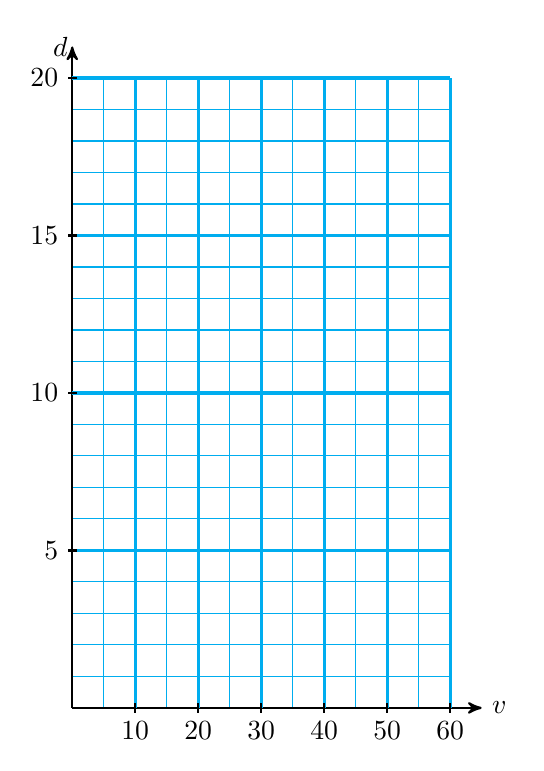
\begin{tikzpicture} [scale=.4]
\draw[cyan] (0,0) grid (12,20);
\draw[black, thick, ->, >=stealth'] (0,0)--(13,0) node[right]{$v$};
\draw[black, thick, ->, >=stealth'] (0,0)--(0,21) node[left,xshift=2]{$d$};
\foreach \x [evaluate=\x as \xi using int(5*\x)] in  {2,4,...,12} {
\draw[cyan, very thick] (\x,0)--++(0,20);
 \draw[black, thick] ({\x},.15) --++(0,-.3) node[below, yshift=-2, fill=white, inner sep=1]   {$\xi$};
}
\foreach \x  in  {5,10,...,20} {
 \draw[cyan, very thick] (0,\x)--++(12,0);
\draw[black, thick] (.15,\x) --++(-.3,0) node[left, xshift=-2, fill=white, inner sep=1]   {$\x$};
}
\end{tikzpicture}
\newline


hp-6-1-30


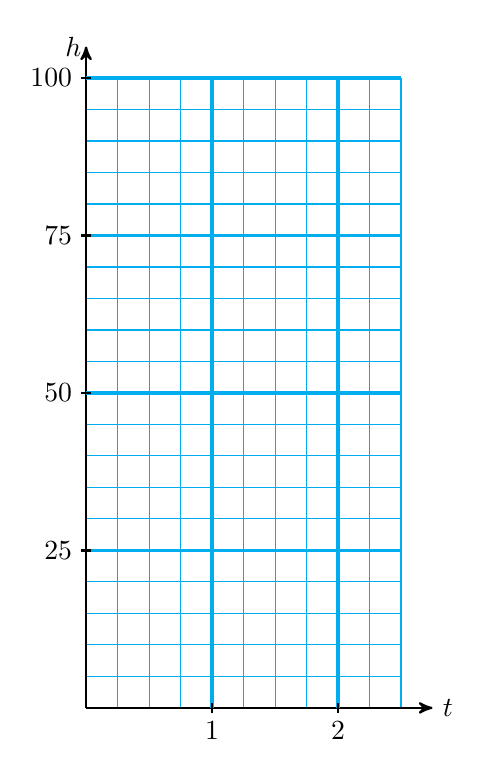
\begin{tikzpicture} [scale=.4]
\draw[cyan] (0,0) grid (10,20);
\draw[black, thick, ->, >=stealth'] (0,0)--(11,0) node[right]{$t$};
\draw[black, thick, ->, >=stealth'] (0,0)--(0,21) node[left,xshift=2]{$h$};
\foreach \x [evaluate=\x as \xi using int(.25*\x)] in  {4,8} {
\draw[cyan, very thick] (\x,0)--++(0,20);
 \draw[black, thick] ({\x},.15) --++(0,-.3) node[below, yshift=-2, fill=white, inner sep=1]   {$\xi$};
}
\foreach \x [evaluate=\x as \xi using int(5*\x)] in  {5,10,...,20} {
 \draw[cyan, very thick] (0,\x)--++(10,0);
\draw[black, thick] (.15,\x) --++(-.3,0) node[left, xshift=-2, fill=white, inner sep=1]   {$\xi$};
}
\end{tikzpicture}
\newline



\section{Section 6.2}



fig-6-2-ex1

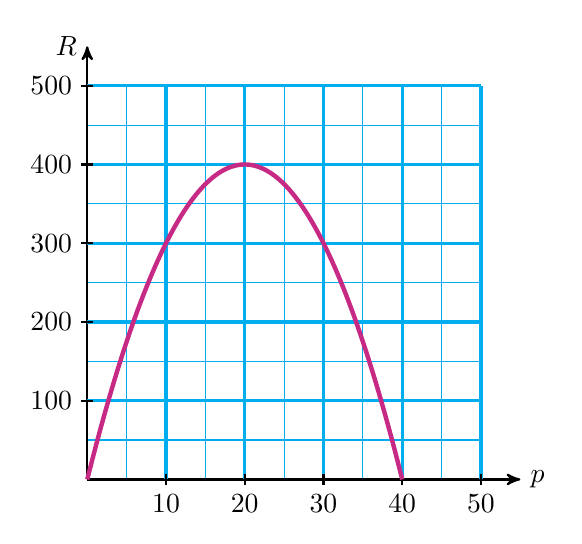
\begin{tikzpicture}[scale=.5]
\draw[cyan] (0,0) grid (10,10);
\draw[black, thick, ->, >=stealth'] (0,0)--(11,0) node[right]{$p$};
\draw[black, thick, ->, >=stealth'] (0,0)--(0,11) node[left]{$R$};
\foreach \x [evaluate=\x as \xi using int(5*\x)] in  {2,4,...,10} {
\draw[cyan, very thick] (\x,0)--++(0,10);
 \draw[black, thick] ({\x},.15) --++(0,-.3) node[below, yshift=-2, fill=white, inner sep=1]   {$\xi$};
}
\foreach \x [evaluate=\x as \xi using int(50*\x)] in  {2,4,...,10} {
 \draw[cyan, very thick] (0,\x)--++(10,0);
\draw[black, thick] (.15,\x) --++(-.3,0) node[left, xshift=-2, fill=white, inner sep=1]   {$\xi$};
}
\draw[samples=65,domain=0:8,smooth,variable=\x,magenta!80!black, ultra thick] plot ({\x},{8-.5*(\x-4)^2});
\end{tikzpicture}
\newline


hp-6-2-25ans 10-by-10 grid

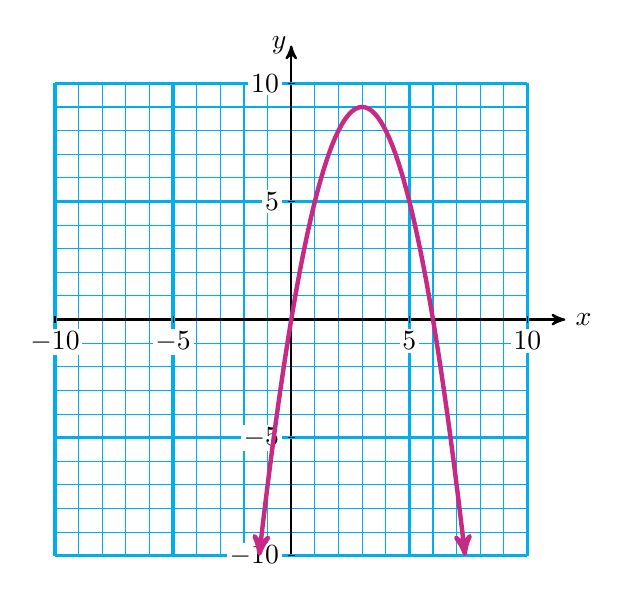
\begin{tikzpicture} [scale=.3]
\coordinate (O) at (0,0);
\draw[cyan] (-10,-10) grid (10,10);
\draw[black,thick, ->, >=stealth'] (-10,0)--(11.6,0) node[right]{$x$};
\draw[black,thick, ->, >=stealth'] (0,-10)--(0,11.6) node[left, xshift=2]{$y$};
\foreach \x in  {-5, 5, -10, 10} {
 \draw[cyan, very thick] (\x,-10) --++(0,20);
 \draw[cyan, very thick] (-10,\x) --++(20,0);
 \draw[black] (\x,.15) --++(0,-.3)  node[below, yshift=-2, fill=white, inner sep=1]   {$\x$};
 \draw[black] (.15,\x) --++(-.3,0)  node[left, xshift=-2, fill=white, inner sep=1]   {$\x$};
}
\draw[samples=65,domain={3-sqrt(19)}:{3+sqrt(19)},smooth,variable=\x,magenta!80!black, ultra thick, <->, >=stealth'] plot ({\x},{-(\x)^2 +6*\x});
\end{tikzpicture}
\newline


hp-6-2-27

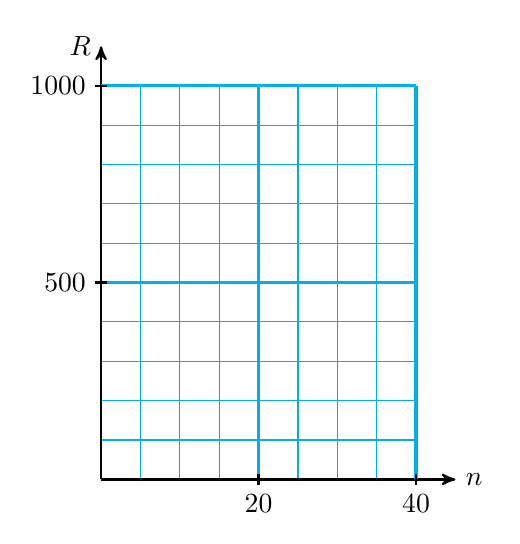
\begin{tikzpicture}[scale=.5]
\draw[cyan] (0,0) grid (8,10);
\draw[black, thick, ->, >=stealth'] (0,0)--(9,0) node[right]{$n$};
\draw[black, thick, ->, >=stealth'] (0,0)--(0,11) node[left]{$R$};
\foreach \x [evaluate=\x as \xi using int(5*\x)] in  {4,8} {
\draw[cyan, very thick] (\x,0)--++(0,10);
 \draw[black, thick] ({\x},.15) --++(0,-.3) node[below, yshift=-2, fill=white, inner sep=1]   {$\xi$};
}
\foreach \x [evaluate=\x as \xi using int(100*\x)] in  {5,10} {
 \draw[cyan, very thick] (0,\x)--++(8,0);
\draw[black, thick] (.15,\x) --++(-.3,0) node[left, xshift=-2, fill=white, inner sep=1]   {$\xi$};
}
\end{tikzpicture}
\newline


hp-6-2-27ans

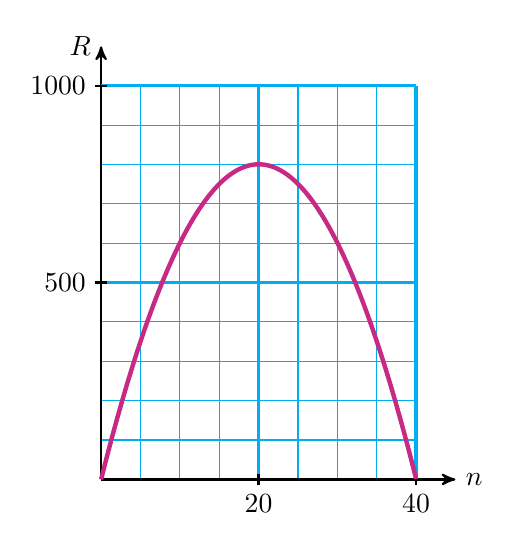
\begin{tikzpicture}[scale=.5]
\draw[cyan] (0,0) grid (8,10);
\draw[black, thick, ->, >=stealth'] (0,0)--(9,0) node[right]{$n$};
\draw[black, thick, ->, >=stealth'] (0,0)--(0,11) node[left]{$R$};
\foreach \x [evaluate=\x as \xi using int(5*\x)] in  {4,8} {
\draw[cyan, very thick] (\x,0)--++(0,10);
 \draw[black, thick] ({\x},.15) --++(0,-.3) node[below, yshift=-2, fill=white, inner sep=1]   {$\xi$};
}
\foreach \x [evaluate=\x as \xi using int(100*\x)] in  {5,10} {
 \draw[cyan, very thick] (0,\x)--++(8,0);
\draw[black, thick] (.15,\x) --++(-.3,0) node[left, xshift=-2, fill=white, inner sep=1]   {$\xi$};
}
\draw[samples=65,domain={0}:{8},smooth,variable=\x,magenta!80!black, ultra thick] plot ({\x},{-1/50*(\x*5)^2 +4*\x});
\end{tikzpicture}
\newline


hp-6-2-28

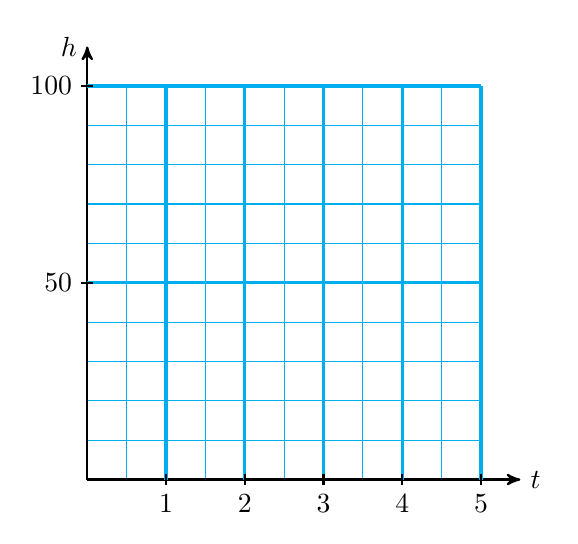
\begin{tikzpicture}[scale=.5]
\draw[cyan] (0,0) grid (10,10);
\draw[black, thick, ->, >=stealth'] (0,0)--(11,0) node[right]{$t$};
\draw[black, thick, ->, >=stealth'] (0,0)--(0,11) node[left]{$h$};
\foreach \x [evaluate=\x as \xi using int(.5*\x)] in  {2,4,...,10} {
\draw[cyan, very thick] (\x,0)--++(0,10);
 \draw[black, thick] ({\x},.15) --++(0,-.3) node[below, yshift=-2, fill=white, inner sep=1]   {$\xi$};
}
\foreach \x [evaluate=\x as \xi using int(10*\x)] in  {5,10} {
 \draw[cyan, very thick] (0,\x)--++(10,0);
\draw[black, thick] (.15,\x) --++(-.3,0) node[left, xshift=-2, fill=white, inner sep=1]   {$\xi$};
}
\end{tikzpicture}
\newline


hp-6-2-29

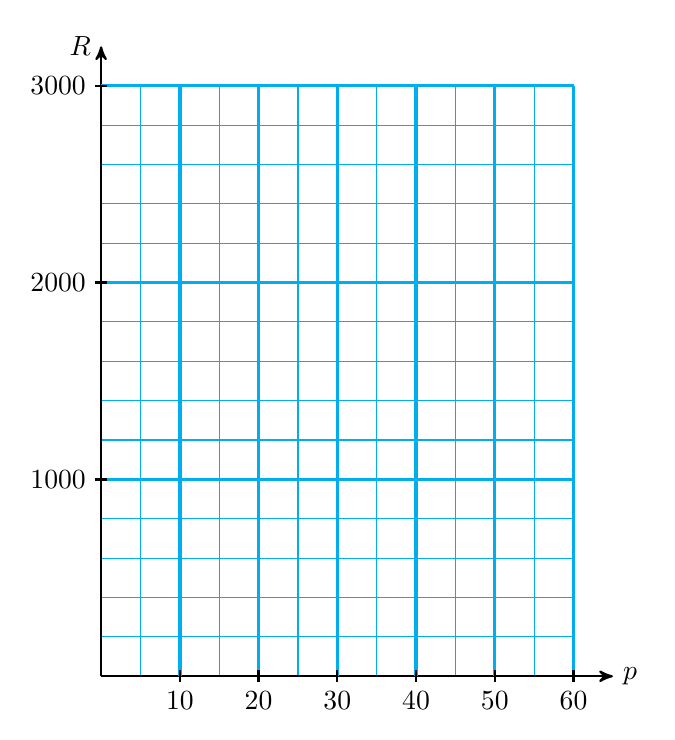
\begin{tikzpicture}[scale=.5]
\draw[cyan] (0,0) grid (12,15);
\draw[black, thick, ->, >=stealth'] (0,0)--(13,0) node[right]{$p$};
\draw[black, thick, ->, >=stealth'] (0,0)--(0,16) node[left]{$R$};
\foreach \x [evaluate=\x as \xi using int(5*\x)] in  {2,4,...,12} {
\draw[cyan, very thick] (\x,0)--++(0,15);
 \draw[black, thick] ({\x},.15) --++(0,-.3) node[below, yshift=-2, fill=white, inner sep=1]   {$\xi$};
}
\foreach \x [evaluate=\x as \xi using int(200*\x)] in  {5,10,15} {
 \draw[cyan, very thick] (0,\x)--++(12,0);
\draw[black, thick] (.15,\x) --++(-.3,0) node[left, xshift=-2, fill=white, inner sep=1]   {$\xi$};
}
\end{tikzpicture}
\newline


hp-6-2-29ans

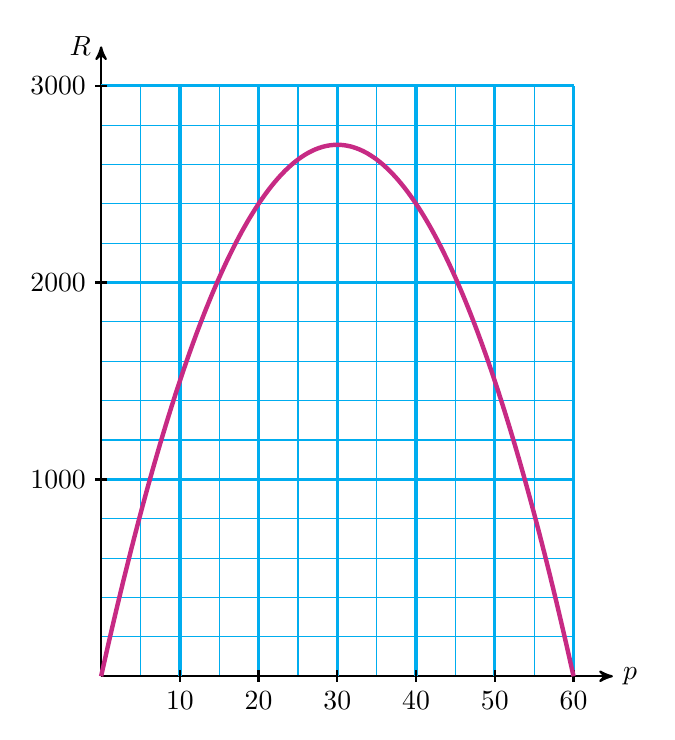
\begin{tikzpicture}[scale=.5]
\draw[cyan] (0,0) grid (12,15);
\draw[black, thick, ->, >=stealth'] (0,0)--(13,0) node[right]{$p$};
\draw[black, thick, ->, >=stealth'] (0,0)--(0,16) node[left]{$R$};
\foreach \x [evaluate=\x as \xi using int(5*\x)] in  {2,4,...,12} {
\draw[cyan, very thick] (\x,0)--++(0,15);
 \draw[black, thick] ({\x},.15) --++(0,-.3) node[below, yshift=-2, fill=white, inner sep=1]   {$\xi$};
}
\foreach \x [evaluate=\x as \xi using int(200*\x)] in  {5,10,15} {
 \draw[cyan, very thick] (0,\x)--++(12,0);
\draw[black, thick] (.15,\x) --++(-.3,0) node[left, xshift=-2, fill=white, inner sep=1]   {$\xi$};
}
\draw[samples=65,domain={0}:{12},smooth,variable=\x,magenta!80!black, ultra thick] plot ({\x},{13.5/36*(\x)*(12-\x});
\end{tikzpicture}
\newline





hp-6-2-33ans 10-by-10 with three curves

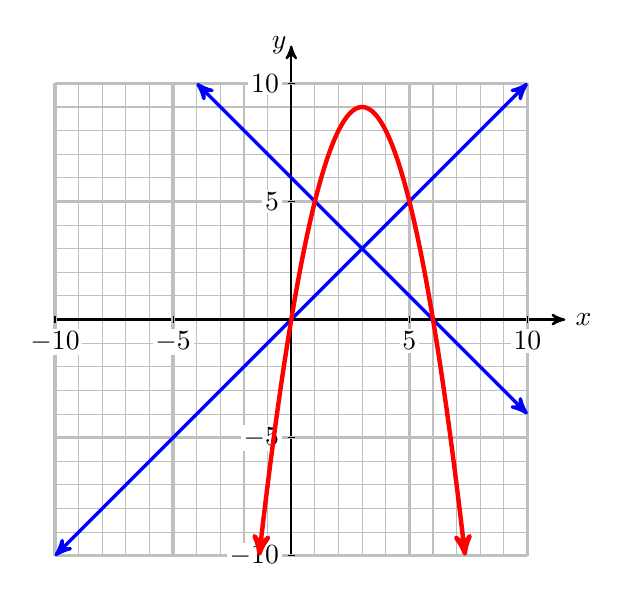
\begin{tikzpicture} [scale=.3]
\coordinate (O) at (0,0);
\draw[lightgray] (-10,-10) grid (10,10);
\draw[black,thick, ->, >=stealth'] (-10,0)--(11.6,0) node[right]{$x$};
\draw[black,thick, ->, >=stealth'] (0,-10)--(0,11.6) node[left, xshift=2]{$y$};
\foreach \x in  {-5, 5, -10, 10} {
 \draw[lightgray, very thick] (\x,-10) --++(0,20);
 \draw[lightgray, very thick] (-10,\x) --++(20,0);
 \draw[black] (\x,.15) --++(0,-.3)  node[below, yshift=-2, fill=white, inner sep=1]   {$\x$};
 \draw[black] (.15,\x) --++(-.3,0)  node[left, xshift=-2, fill=white, inner sep=1]   {$\x$};
}
\draw[blue,very thick, <->, >=stealth'] (-10,-10)--(10,10);
\draw[blue,very thick, <->, >=stealth'] (-4,10)--(10,-4);
\draw[samples=65,domain={-sqrt(19)+3}:{sqrt(19)+3},smooth,variable=\x,red, ultra thick, <->, >=stealth'] plot ({\x},{6*\x - (\x)^2});
\end{tikzpicture}
\newline





\section{Section 6.3}



fig-6-3-1 subdivided rectangle

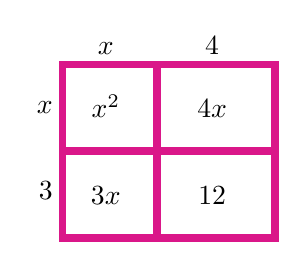
\begin{tikzpicture} 
\draw[magenta!90!black, line width=1mm] (0,0) rectangle ++(2.7,2.2);
\draw[magenta!90!black, line width=1mm] (0,1.1) --++(2.7,0);
\draw[magenta!90!black, line width=1mm] (1.2,0) --++(0,2.2);
\node[above] at (.55,2.2) {$x$};
\node[above] at (1.9,2.2) {$4$};
\node[left] at (0,1.65) {$x$};
\node[left] at (0,0.6) {$3$};
\node[above] at (0.55,1.4) {$x^2$};
\node[above] at (1.9,1.4) {$4x$};
\node[above] at (0.55,.3) {$3x$};
\node[above] at (1.9,.3) {$12$};
\end{tikzpicture}
\newline


fig-6-3-2

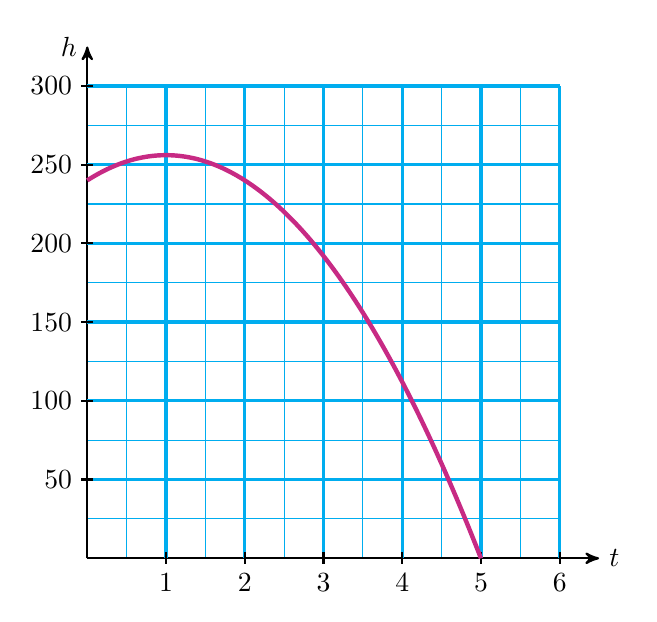
\begin{tikzpicture}[scale=.5]
\draw[cyan] (0,0) grid (12,12);
\draw[black, thick, ->, >=stealth'] (0,0)--(13,0) node[right]{$t$};
\draw[black, thick, ->, >=stealth'] (0,0)--(0,13) node[left]{$h$};
\foreach \x [evaluate=\x as \xi using int(0.5*\x)] in  {2,4,...,12} {
\draw[cyan, very thick] (\x,0)--++(0,12);
 \draw[black, thick] ({\x},.15) --++(0,-.3) node[below, yshift=-2, fill=white, inner sep=1]   {$\xi$};
}
\foreach \x [evaluate=\x as \xi using int(25*\x)] in  {2,4,...,12} {
 \draw[cyan, very thick] (0,\x)--++(12,0);
\draw[black, thick] (.15,\x) --++(-.3,0) node[left, xshift=-2, fill=white, inner sep=1]   {$\xi$};
}
\draw[samples=65,domain=0:10,smooth,variable=\x,magenta!80!black, ultra thick] plot ({\x},{240/25+16/25*\x-16/25*(\x/2)^2});
\end{tikzpicture}
\newline


hp-6-3-33

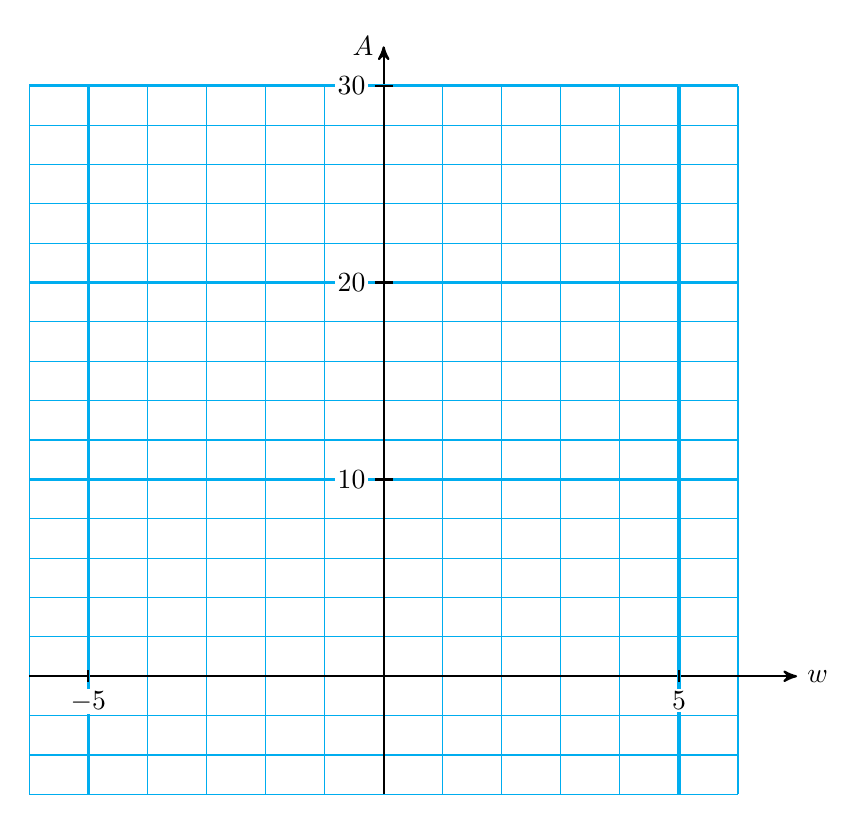
\begin{tikzpicture}[xscale=.75, yscale=.5]
\draw[cyan] (-6,-3) grid (6,15);
\draw[black, thick, ->, >=stealth'] (-6,0)--(7,0) node[right]{$w$};
\draw[black, thick, ->, >=stealth'] (0,-3)--(0,16) node[left]{$A$};
\foreach \x in {-5,5} {
 \draw[cyan, very thick] (\x,-3)--++(0,18);
 \draw[black, thick] (\x,.15) --++(0,-.3) node[below, yshift=-2, fill=white, inner sep=1]   {$\x$};
}
\foreach \x [evaluate=\x as \xi using int(2*\x)] in  {5,10,15} {
 \draw[cyan, very thick] (-6,\x)--++(12,0);
\draw[black, thick] (.15,\x) --++(-.3,0) node[left, xshift=-2, fill=white, inner sep=1]   {$\xi$};
}
\end{tikzpicture}
\newline


hp-6-3-33ans

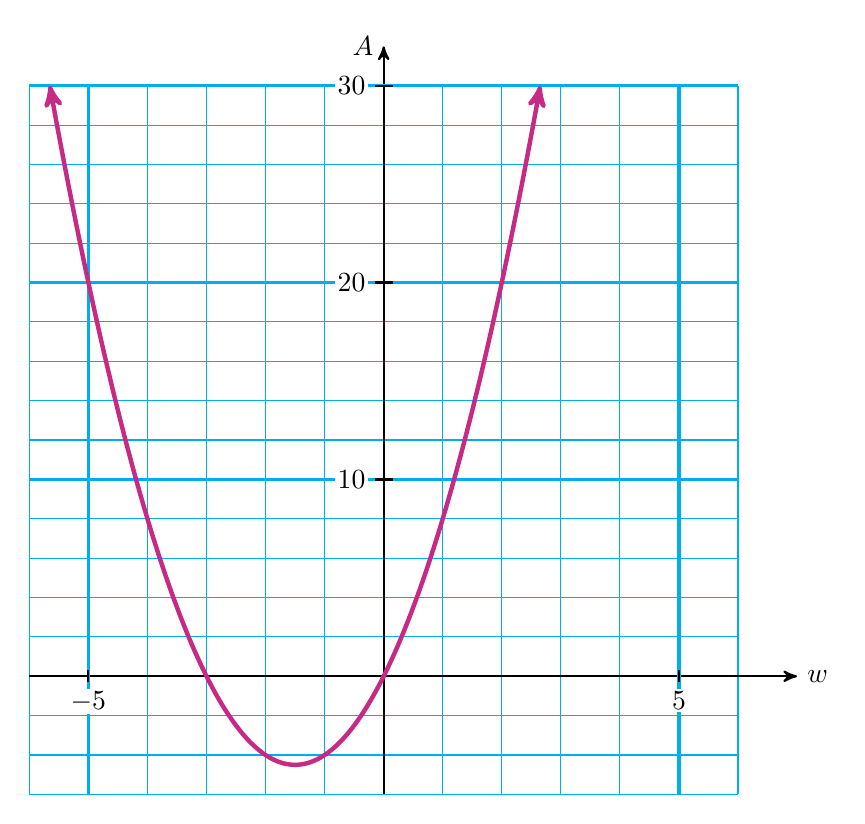
\begin{tikzpicture}[xscale=.75, yscale=.5]
\draw[cyan] (-6,-3) grid (6,15);
\draw[black, thick, ->, >=stealth'] (-6,0)--(7,0) node[right]{$w$};
\draw[black, thick, ->, >=stealth'] (0,-3)--(0,16) node[left]{$A$};
\foreach \x in {-5,5} {
 \draw[cyan, very thick] (\x,-3)--++(0,18);
 \draw[black, thick] (\x,.15) --++(0,-.3) node[below, yshift=-2, fill=white, inner sep=1]   {$\x$};
}
\foreach \x [evaluate=\x as \xi using int(2*\x)] in  {5,10,15} {
 \draw[cyan, very thick] (-6,\x)--++(12,0);
\draw[black, thick] (.15,\x) --++(-.3,0) node[left, xshift=-2, fill=white, inner sep=1]   {$\xi$};
}
\draw[samples=65,domain={-sqrt(69)/2-3/2}:{sqrt(69)/2-3/2},smooth,variable=\x,magenta!80!black, ultra thick, <->, >=stealth'] plot ({\x},{\x*(\x+3)});
\end{tikzpicture}
\newline



\section{Other stuff}

10 by 10 grid: hp-2-3-12

8 by 8 grid: hp-4-5-17



\end{document}
